Um ein besseres Verständnis zu ermöglichen, wird zunächst auf die generelle Funktionsweise von Maven näher eingegangen. 

\subsubsection{Workflow Maven}
Maven verfolgt die Philosopie \textit{Konvention über Konfiguration}. 

In diesem Rahmen sind Strukuren oder Abläufe, die zur Kompilierung, Testen, Paketierung und Veröffentlichung von Projekten benötigt werden, bereits vorgegeben und müssen nicht mehr definiert werden, wodurch sich die Entwicklung auf den Inhalt des Projektes einschränkt. \cite[S. 27]{spiller_maven_2011}

Softwareentwickler werden unterstützt, indem Maven die Ordnerstruktur und Organisation eines Projektes standardisiert und Empfehlungen abgibt, wo sich verschiedene Teile des Codes wie der Quellcode oder Konfigurationsdateien abgelegt werden sollten. \cite[S. 2]{varanasi_introducing_2019}  

Ferner bietet Maven die Möglichkeit Projektabhängigkeiten, Projektumgebungen und Projektbeziehungen in einer seperaten, externen pom.xml-Datei zu deklarieren. \cite[S. 3]{varanasi_introducing_2019} 

Dies erleichtert insbesondere die Verwaltung von Projektabhängigkeiten, da Bibliotheken einfach ausgetauscht werden können und die entsprechenden Abhängigkeiten sowie die transitiven Abhängigkeiten aufgelöst und entfernt werden.

Aufgrund der vielen automatisierten und standardisierten Schritte insbesondere im Bereich des Build-Managements, wird die Navigation übersichtlich und das Verständnis erheblich erleichtert. 

\begin{figure}[h]
    \centering
    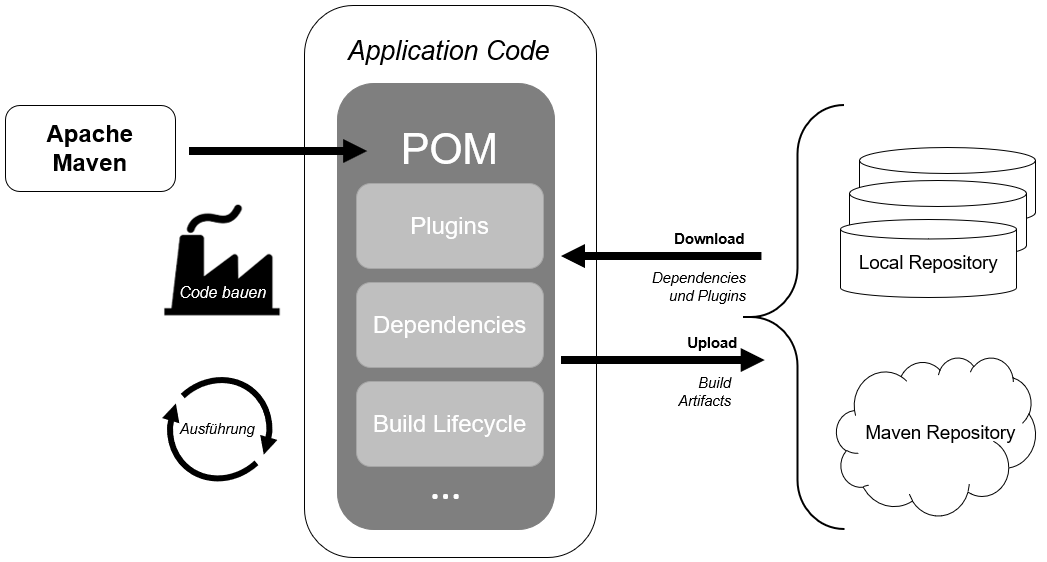
\includegraphics[scale=0.6]{Bilder/Workflow_Maven.png}
    \caption{Funktionsweise von Maven, angelehnt an \cite{guntur_understanding_2020}}
\end{figure}

\paragraph{POM}
Die Funktionsweise von Maven als auch die Verwaltung des Projektes baut grundsätzlich auf dem 'Project Object Model' (kurz: POM) auf und bildet daher den Kern eines jeden Maven-Projektes ab.

Die POM wird innerhalb der Datei pom.xml gespeichert, die wiederrum im Projektverzeichnis liegt.

Die POM beinhaltet alle notwendigen Projektinformationen, vorhandenen Abhängigkeiten, dem Quelldateiverzeichnis Konfigurationen und Plugininformationen, die während des Build-Prozesses verwendet werden sollen.\cite{the_apache_software_foundation_maven_2002}

Die POM muss drei wesentliche Tags enthalten \cite[S. 77 - 78]{spiller_maven_2011}: 

\begin{itemize}
    \item \textit{groupId}: Enthält eine eindeutige, identifizierbare Bezeichnung für ein Projekt
    \item \textit{artifactId}: Enthält eine eindeutige, identifizierbare Bezeichnung für ein Artefakt bzw. Projekt pro groupId
    \item \textit{version}: Enthält die aktuelle Version des Artefakts
\end{itemize}

Alle weiteren definierten Eigenschaften werden von der Super-POM vererbt, welches die Standardkonfigurationen, Plugins und Verzeichnisse enthält.

Entscheidend ist, dass Maven keine vollständigen Projekte, sondern eigenständige Projektteile, also Artefakte beschreibt, die einzeln ausgeliefert werden. \cite[S. 29]{spiller_maven_2011}

Demzufolge erzeugt jedes Maven-Projekt ein Artefakt, welches auf die Repositorys übertragen wird. 

\paragraph{Repository}

Ferner verwendet Maven das 'Local Repository' und das konfigurierte 'Maven Repository'.

Innerhalb des Local Repositorys werden alle Abhängigkeiten abgelegt, die für die Erstellung des Builds benötigt werden. 

Zunächst überprüft Maven bei der Zerlegung der Abhängigkeiten, ob sich die benötigten Dateien bereits innerhalb des Local Repositorys befinden. \cite[S. 45 - 47]{loukides_maven_2008} 

Ist dies der Fall, wird die Datei, ohne die Erstellung einer Kopie im lokalen Verzeichnis, innerhalb des Local Repositorys verwendet.

Kann keine Zerlegung der Abhängigkeiten lokal erfolgen, versucht Maven diese mittels dem Maven Repository über das Internet auf das Local Repository herunterzuladen und zu kopieren, damit diese aussschließlich lokal verwendet werden. \cite[S. 115]{spiller_maven_2011}   

Sollten neue Abhängigkeiten oder neue Versionen der vorhandenen Abhängigkeiten hinzugefügt werden, wird das Repository anhand dessen aktualisiert oder die betreffenden Abhängigkeiten kopiert. 

Die Abhängigkeiten, also die genutzten Bibliotheken werden in der pom.xml definiert. 

\paragraph{Build-Lifecycle}

Prinzipiell sind Lifecycles abstrahierte Arbeitsschritte innerhalb festen Phasen, die in einer bestimmten Reihenfolge durchlaufen und für den Build-Prozess essentiell sind. \cite[S. 57]{varanasi_introducing_2019}  

Durch das standardisierte Vorgehen, lässt sich das Ararbeiten der Aufgaben verallgemeinern und vereinheitlichen, was für den Entwickler unterstützend ist.

Maven definiert dabei drei Lifecycles\cite[S. 72 - 76]{spiller_maven_2011}: 

\begin{itemize}
    \item \textit{clean}\\
    Mittels dieses Lifecycles wird alles gelöscht, was keine Notwendigkeit mehr hat, so wie beispielsweise die vom vorherigen Build erstellten Dateien. 

    \item \textit{site}\\
    Innerhalb dieses Lifecycles umfasst alle Phasen, die zum Erzeugen einer Projektdokumentation benötigt werden.
    
    \item \textit{build/default}\\
    Dieser Lifecycle stellt den standardisierten Ablauf aller Phasen dar, die nach dem Aufruf von Maven zum Übersetzen und Erzeugen einer Anwendung abgearbeitet werden. 
    
    Dieser enthält acht wesentliche Phasen, die nach einer unveränderbaren Reihenfolge abgearbeitet werden: validate, compile, test, package, integration-test, verify, install und deploy.  

\end{itemize}

Folglich muss bei einem Aufruf einer bestimmten Phase, die vorangegangen Phasen ebenfalls abgearbeitet werden. 

Neben den Phasen sind auch die zugrundeliegenden Plugins innerhalb jedes Lifecycles verbunden, die sich wiederrum durch das Ausführen von Plugin-Goals in den einzelnen Phasen modefizieren lassen. \cite[S. 71]{spiller_maven_2011}

\begin{figure}[h]
    \centering
    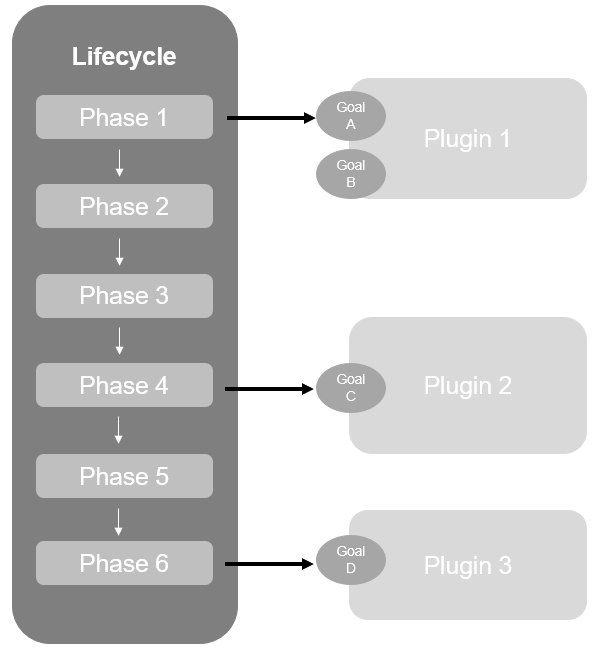
\includegraphics[scale=0.6]{Bilder/lifecycle_maven.png}
    \caption{Zusammenspiel Plugin-Goals und Lifecycle, \cite[S. 59]{varanasi_introducing_2019}}
\end{figure}

Sobald Maven die einzelnen Phasen eines Lifecycles durchläuft, werden die Ziele ausgeführt, die mit jeder einzelnen Phase verbunden sind. \cite[S. 39]{loukides_maven_2008} 

Infolgedessen werden bestimmte Funktionalität eines Plugins durch das entsprechende Goal bestimmt. 

Während das POM alle notwendigen Informationen über ein Projekt enthält, die während des Build-Prozesses verwendet werden sollen, also das "Wer", "Was" und "Wo", stellt der Lifecycle das "Wann" und "Wie" dar. \cite{the_apache_software_foundation_maven_2002}

\paragraph{Plugins in Maven}

Wie bereits beschrieben, ist Maven ein Framework zum Ausführen von Plugins, indem benötigte Funktionen als Plugins anhand des Goals in den Softwareentwicklungsprozess ausgeführt werden.

In diesem Rahmen wird das Konzepts \textit{Seperation of Concerns} verfolgt. 

Aufgrund der hohen Anzahl der Varianten derselben Funktionalitäten wie beispielsweise das Kompilieren oder das Testen, muss stets ein Goal innerhalb eines Plugins angegeben werden, wodurch ein Maven-Plugin für genau eine Aufgabe zuständig ist. 

Infolgedessen kann jede Funktionalität durch ein Plugin ersetzt werden, wodurch Plugins eine zentrale Rolle innerhalb des Softwareentwicklungsprozesses zufällt. 

Wird das Plugin regelmäßig verwendet, wird dieses innerhalb der POM deklariert, ansonsten reicht ein Aufruf über die Kommandozeile.  

Durch die Koordinaten groupId, artifactId und version können die Artefakte identifiziert werden, wobei die Verwaltung der Abhängigkeiten ebenfalls im Repository erfolgt. 

Mittels der Auslagerung unterschiedlicher Aufgaben, ist sowohl der Einsatz als auch die Wartung einfacher wie bei großen Abhängigkeiten, da die Aktualisierung durch Maven durchgeführt werden.  

\subsubsection{Entwurf PoC basierend auf einem Maven-Plugin}
%Idee: Lizenzen als eine Datei zu beschreiben und mit den Lizenzen die sich in den Dependency-Dateien befinden, zu vergleichen 




